\providecommand{\sixbysix}{\ensuremath{6\times 6\mathrm{~cm}^{2}}\xspace}
\providecommand{\threebythree}{\ensuremath{3\times 3\mathrm{~cm}^{2}}\xspace}
\providecommand{\twobytwo}{\ensuremath{2\times 2\mathrm{~cm}^{2}}\xspace}
\providecommand{\onebyone}{\ensuremath{1\times 1\mathrm{~cm}^{2}}\xspace}

\chapter{The HL-LHC upgrade of CMS}
\label{chapter:cms_upgrade}

In this chapter the upgrade of the LHC complex is briefly introduced in Section~\ref{upgrade_lhc}
underlining the physics goal and the expected performace of the machine. The CMS experiment is already planning
a series of upgrades, most of which will be installed during LS3 (Figure~\ref{fig:lhc_plan}).
The overall goal of the CMS upgrade is introduced in  while
further details on the upgrade of the CMS ECAL are reported in the rest of the chapter.
The ECAL upgrade mainly concerns the read-out electronics and trigger system, these are introduced in Section ??
while in Section ??.

\section{High Luminosity LHC}
\label{upgrade_lhc}

The main objective of the High Luminosity LHC (HL-LHC) upgrade [9] of the LHC accelerator complex
is to make precise measurements of the Higgs boson couplings, the standard model and provide a very
large dataset ($3000\fbinv$) for new physics searches.
The design include a substantial upgrade of the accelerator complex with the goal of reaching
a peak luminosity of $7.5\times10^{34} cm^{-2}s^{-1}$ (roughly four times as mush as the current value)
The integrated luminosity will about ten times the expected luminosity of the first twelve
years of the LHC.
The timeline of LHC and HL-LHC operation is sketched in Figure~\ref{fig:lhc_plan}, showing the planned
evolution of proton beam intensity through the remaining LHC operating periods (Run 2 and Run 3)
and the HL-LHC operating period following the upgrade of the accelerator complex in LS3.
%The two periods of operation are termed Phase-1 (LHC) and Phase-2 (HL-LHC).

The peak luminosity will be achieved by increasing the beams intensities and by squeezing more the two beams at the
interaction points. This will lead to a higher number of collisions occuring within the same bunch crossing, the
average number of collisions will increase from 40-60 of LHC to 140-200 at HL-LHC.
The ability of the detectors (ATLAS and CMS) in assagning particles to the correct collision will worsen with the
increased instantaneous luminosity expetially for energy deposits in the calorimeters.


\section{HL-LHC upgrade of CMS}
\label{upgrade_cms}
The CMS detector will be upgraded to match the operation environment of HL-LHC in order to fully exploit the
larger dataset delivered by the accelerator complex.
The major points are
the replacement of the entire calorimeters system in the endcaps to cope with the expected level of radiation
of HL-LHC (more than $1.5\times10^{15} n_{eq}/cm^{2}$ in the parts closer to the beam line),
the complete replacement of the Level-1 trigger and the proposed installation of a new detector to measure the
time of charged particles with a precision of about $30 ps$. These three major points also drives upgrades of
the other existing components: the upgrade of the Level-1 trigger will profit from an extended
muon system coverage up to $|\eta| = 2.8$, new tracker system cabable of providing information at
Level-1 and calorimeter system electronics upgraded to match the trigger rate allowed by the Level-1.
The completely new calorimenter system in the endcaps will provide longitudinal shower development which will
in turn improve descimination between energy deposits coming from different collisions.
Finally the time information extracted with the new system will be matched by those of the ECAL barrel and the new
endcap calorimeter. The ECAL si expected to provide a time information on electromagnetic showers
with a precision of $30 ps$ for energies above few tens of GeV.

\section{The ECAL barrel upgrade}
The primary technical motivation for the ECAL barrel (EB) upgrade is the trigger requirement for
an increase of the trigger latency from about $4\mu$s in the current system [4] to a maximum of $12.5\mu$s,
and a Level-1 trigger rate of up to 750 kHz compared to the current 100 kHz.
The EB electronics Front End (FE) card and all the read-out electronics will be replaced to
meet these requirements. The current configuration provides trigger information to the Level-1
with a granularity of five-by-five crystals, the upgraded system will have a single crystal granularity
enhanching event selection based on isolation information at trigger level which will in turn allow
to set lower thresholds on the transverse energy of the candidate particles.

The foreseen upgraded FE electronics will also provide a shape discrimination between
signal compatible with an electromagnetic shower and those originated from hadronic interaction (``spikes'') in
the photodetector (APD) which have a narrower shape. The increased Level-1 granularity of a single crystals
will also improve the rejection of such events at trigger level.
The shape discrimination is made possible by a shorter signal shaping performed by the amplification chain
coupled with a signal sampling frequency of 160 MHz (four times the current). The increased sampling
frequency is also the key upgrade to provide a time measurement at the $30 ps$ level (Section ??) and
is limited by overall CMS constrain on data transfer bandwidth and power consumption.

% \subsection{The ECAL timing performance}
% To assess the timing capabilities of the ECAL a series of test beams have been carried out during the R\&D phase.
% The test beam goal is to first measure the intrinsic time resolution achievable with \PbWO crystals and
% APD system and at a second stage verify the performance with the sampling frequency of 160MHz.

\subsection{The current ECAL timing performances}
The time of an electromagnetic shower in the ECAL is defined as the time at which the signal generated
in the APDs reachs its maximum amplitude. The method to extract this information for the digitized signal
shape is described in \cite{ecal_time_reco}. The time of the maximum $T_{max}$ is estimated with each
available pair of samples (up to nine) as:
\[
T_{max, i} = T_i - T(R_i)
\]
where $i$ is the $i-th$ sample, $T_i$ is acquisition time of the $i-th$ sample and $T(R_i)$ is the time
corresponding to the amplitude ratio $R_i = A_i/A_{i+1}$ and is extracted from a parametrization whose parameters
were measured in a test beam prior the installation of CMS. The error ($\sigma_i$) on each $T_{max, i}$ is estimated as
the product of the derivative of the $T(R)$ function and the uncertainty on $R_i$ which is the sum in quadrature
of three components: noise fluctuations in each sample, uncertainty on the pedestal value subtracted from the measured amplitued
and trunction occuring during the 12 bit digitization of the amplitude.
For signal syncronized with the LHC bunch crossing only four or five of the nine possible amplitude
ratios are used, samples with very small amplitude are discarded. The unique signal time is computed
as the weighted average of the  $T_{max, i}$:
\[
  T_{max} = \frac{\sum_i T_{max, i}/\sigma_i^2}{\sum 1/\sigma_i^2}
\]
and the its error as:
\[
  \frac{1}{\sigma_{T_{max}}^2} = \sum_i\frac{1}{\sigma_i^2}
\]

The time resolution can be parametrized as:
\begin{equation}
  \sigma^2(t) = \left( \frac{N\cdot\sigma_n}{A} \right)^2 + \left( \frac{S}{\sqrt{A}} \right)^2 + C^2  
\end{equation}
\label{eq:general_time_res}

where A is the measured signal amplitude, $\sigma_n$ is the RMS of the noise for each sample and
N, S, C represent the noise, stochastic, and constant term coefficients, respectively.
The stochastic term S is related to fluctuations in the colletion times of scintillation photons due to
the finite time their emission.

% It was verified in \cite{ecal_time_reco} to have a negligible impact on
% the time resolution expetially when looking at the time difference for two crystals hit by the same electromagnetic
% shower . 

The time performance of the ECAL has been estimated both during the pre-installation test beam \cite{ecal_time_reco}
and with data collected during the 8 TeV operation of LHC \cite{delRe_time_ecal}.
In the test beam measurement the resolution was extracted from the time difference between the two most energetic crystals
af the same electromagnetic shower, in this configuration the stochastich term that appears in Equation~\ref{eq:general_time_res}
can be neglected since shower flactuation effects cancels out in the difference, Equation~\ref{eq:general_time_res} thus becomes:
\begin{equation}
  \sigma^2(t_1 - t_2) = \left( \frac{N\cdot\sigma_n}{A_{eff}} \right)^2 + 2 \cdot C^2
\end{equation}
\label{eq:ecal_time_res}
Where $A_{eff} = A_1A_2/\sqrt{A_1^2+A_2^2}$ and $t_{1,2}$, $A_{1,2}$ refers to the times and amplitudes measured by the two crystals. 
The time resolution $\sigma(t_1-t_2)$ was estimated with a gaussian fit to the time difference.
The results obtained in the analysis report a constant term of $20 \pm 4$ ps which, together with a noise term $N = 35.1\pm 0.2$ ns,
gives and expected time resolution better than 100 ps for energy deposits greater than 20 GeV in the barrel.

The prediction was tested wih data collected during 2011 and 2012 from CMS. With collisions events it is possible to
test the performance of the whole system including the clock distribution. \Zee events where used in \cite{delRe_time_ecal}
the results show a good performance when measuring the time difference for channels belonging to the same readout unit while
an increasingly poorer performance for channels in different readout units but same shower and channels belonging to
the two different superclusters in \Zee events (Figure~\ref{fig:ecal_runI_time}).

\begin{figure}[h!]
  \centering
  \includegraphics[width = 0.45\textwidth]{figures/upgrade/t_res_sameRO.pdf}
  \includegraphics[width = 0.45\textwidth]{figures/upgrade/t_res_diffRO.pdf}\\
  \includegraphics[width = 0.5\textwidth]{figures/upgrade/ecal_resol_Z.pdf}
  \caption{Resolution of time difference between the two most energetic crystals of an ECAL cluster as a function of the
    effective amplitude $A_{eff}$, normalized to the noise in the ECAL Barrel for 2011+2012 data,
    for crystals belonging to the same readout unit (top left), different readout unit (top right) and the two most
    energetic crystals in each of the superclusters generated by electron from \Zee decays (bottom).
    For electrons from Z boson decays the time of each crystals is corrected for the time of flight from the common
  interaction vertex.}
  \label{fig:ecal_runI_time}
\end{figure}

These results were interpreted to be due to time jitter introduced by the clock distribution system and not corrected by
the calibration performed with low energy deposits. The clock stability has been measured in 2016 using laser monitoring data
and while the time resolution constant term is found to be below $40 ps$ even for crystals belonging to different readout unit,
instabilities of the clock syncronization at the level of $100 ps$ were observed over the course of few days. The
observed effect is in agreement with the constant term measured using \Zee events that are collected over a long period of time.

\subsection{Test beam results with HL-LHC electronics}
During 2015 and 2016 a series of tests with electron beam were performed to evaluate the time performance
of the \PbWO crystal plus APDs photodetectors system (2015 beam test, Section~\ref{sec:tb_2015})
and that of the proposed HL-LHC ECAL electronics (2016 beam test, ??).
The tests differ from the ones conducted before the CMS installation since the time of the electron measured by the
crystal is compared to an external reference provided by a multi-channel-plate based detector (MCP) instead of to an adiacent
crystal hit by the some shower.

\subsubsection{Test beam setup}
\label{sec:tb_2015}
The first test was conducted in 2015 at the CERN SPS north area with a tunable beam of electrons with energies between 20 and 250 GeV.
The electron beam is a secondary beam created from the primary proton beam, extracted from the SPS, using a conveter.
The primary beam hits a metallic target producing a variety of particles that are selected through a system of magnets, collimators
and additional targets. The beam line used for the tests can reach a electron purity of $99\%$ and can also be
configured to provide a equally pure pion beam to study ``spikes'' in the APDs.
The beam in the SPS is composed of several bunches that are extracted in an interval of 4-5 s every 14-48 s depending on the
SPS cycle configuration. The extraction line is configured in a way to destroy the bunch scheme of the SPS beam in order
to provide a uniform and less intense beam to the test area.
The energy of the secondary beams of electrons, positron, muons and charged pions can be selected within the 10 to 400 GeV
range. 

The experimental setup included a $5\times 5$ \PbWO crystal matrix identical to those installed in the ECAL barrel,
with two APDs glued at the back (A schematic view of the setup is shown in Figure~\ref{fig:tb_setup}.
The APDs signals were amplified with the same $CR-RC$ circuit installed in the current ECAL
supermodules, the shaping time for some of the channels was set to 21.5 ns (half of the current one) to match the
one proposed for the HL-LHC upgrade.
The amplified signal was digitized with a 5 GSample/s commercial digitizer (CAEN V1742 VME board)
instead of the final design
DAC with 160 MHz sampling frequency.
In order to estimate the impact of fluctuation in the light production depth on the time resolution,
two of Silicon photon multipliers (SiPM) arrays were glued to the front face of the central crystal.
The CAEN digitizer was used to readout also the signals two of SiPM.

The crystal matrix and readout electronics was kept at $18^{\circ}$ inside box to avoid
light indeced noise in the photodetectors. The reference MCP detector was placed in front of the box. 
Incoming charged particles produce cherenkov radiation in a quartz window coupled to a photocathode,
the photoelectrons produced by the cherenkov light hitting
the photodathode are amplified by two layers of MCP and collected to the anode. 
The MCP device used in the test was caracterized 
in a different test [??] and its time resolution measured to be 25 ps constant for electron energies
above 20 GeV. The signal from the MCP was also digitized with the same CAEN board.

\begin{figure}[h!]
  \centering
  \includegraphics[width = .7\textwidth]{figures/upgrade/tb_setup.pdf}
  \caption{Schematic of the beam test setup (not to scale), the electron beam comes from the left side.
    The \PbWO crystal is drawn in green and the shape is simplified with
    respect the real trapezoidal one. The plastic scintillators described in the text are not drawn and were placed
    upstream of the hodoscope (to the left of HODO in the picture). As in the standard ECAL crystals the signals from the two APDs
    eglued on the rear face are merged before the preamplifier (VFE in the scheme).}
  \label{fig:tb_setup}
\end{figure}
  
The setup was complemented by a set of wire chambers and scintillating fibers hodoscopes to measure the position in the plane
transverse to the beam direction (x-y plane) of particles hitting the experimental setup.
Each hodoscope is composed by a set of 64 fibers and has a spatial resolution of 0.5 mm and was placed
3 meter upstream of the crystals box and the MCP. The beam divergence is negligible and thus the impact point on the crystals
face corresponds to the particle transverse position measured by the hodoscopes (Figure~\ref{fig:crystal_amp_map}).

Incoming particles were also detected by three plastic scintillators placed few meters upstream of the crystals position, the
three scintillation signal are discriminated and a trigger for the acquisition system is build as a coincidence of the three signals.
The three scintillators diminsions are \sixbysix, \threebythree, \onebyone, the smallest one selects event impinging at the
center of the \twobytwo crystal front face.

\begin{figure}[h!]
  \centering
  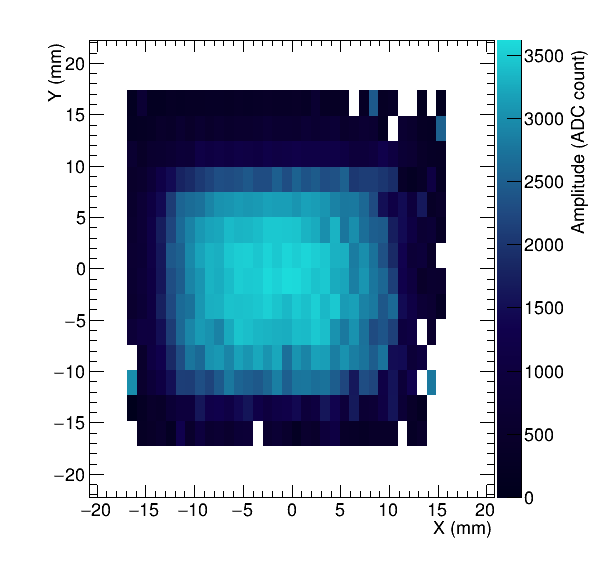
\includegraphics[width = 0.7\textwidth]{figures/upgrade/crystal_amp_map.pdf}
  \caption{Distribution of the signal amplitude of a single crystals as a function of the transverse inpact position for
    a 50 GeV electron beam. For alignment porpouses the events shown in the picture
    were acquired requiring only the coincidence between the \sixbysix and \threebythree scintillators.
    The crystal front face is a square with 22 mm sides, the area covered by the crystal is clearly visible in the amplitude
    profile as the light area at the center.}
  \label{fig:crystal_amp_map}
\end{figure}

\subsubsection{Amplitude and time reconstruction at the beam test}
The CAEN digitizer has 32 channels and for each event and channel acquires 1024 samples (one every 200 ns). The
digital conversion is performed by a 12-bit DAC, the dynamic range of the DAC is 1 V.
The channels are syncronized at a level better than 5 ps.
The samples were shipped to a commercial PC through the VME bus and an optical interface, the event
syncronization between the digitizer, hodoscopes and wire chamber data was performed by software running on the
acquisition PC.

The MCP signal is very fast, lasting 4 ns, its amplitude is estimated with a second order polinomial fit to the seven samples
around the maximum one while the time extracted with a constant fraction method to avoid amplitude walk effects.

The signal from the SiPM is readout through a NINO chip that provides both the time and amplitude measurements.
The signal time is extracted with a precision under 10 ps as the the time at which the signal pass a threshold that
can be configured. This method is very sensibile to the amplitude walk effect and the measured time is therefore
corrected during the analysis.

The amplitude and time of the APD signal are estimated with a template fit to the signal shape where the signal
amplitude and time of the maximum are free to float.
The template shape is build as the average of $1\times 10^5$ signals aligned using the time of the MCP signal
in the same event and scaled by the amplitude estimeted with the same approach used for the MCP signal.
A different template shape is constructed in this way
for each crystal. Two template examples are shown in Figure~\ref{fig:apd_templates} for channel with different  
shaping times. The template fit gives the best time performance for APD signals which has a smaller $dV/dt$ compared
to the MCP one.

\begin{figure}
  \centering
  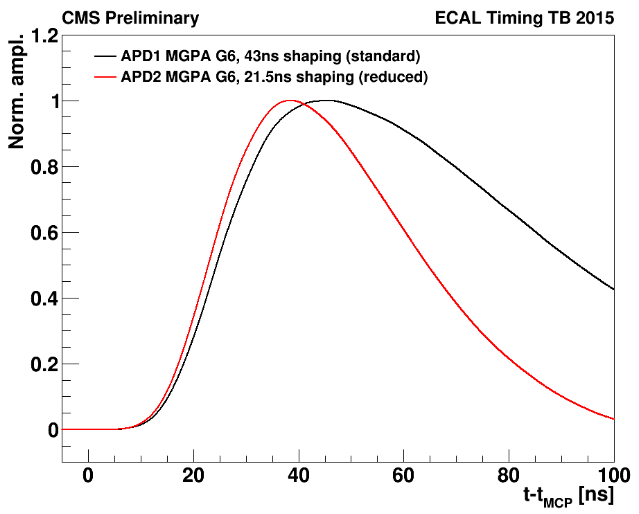
\includegraphics[width = 0.7\textwidth]{figures/upgrade/wf_shaping_times.png}
  \caption{APD signal average shape for 21.5 ns and 43 ns shaping times.}
  \label{fig:apd_templates}
\end{figure}

\subsubsection{Beam test results}
The resolution of the \PbWO crystals plus APDs system is extracted from 
the distribution of the time difference between the time measured by the MCP ($t_{MCP}$) and the crystal ($t_{APD}$)
hit by the electron.
A gaussian function is fit to the distribution and the standard deviation extracted from the fit is quoted as
the time resolution. The operation is performed at different energies and for two channels with different
amplifier shaping times. Only events in which the electron entered the crystal within 1.5 mm from the center of the
front face where selected. 

Figure~\ref{fig:results_treso} shows the results for the two different shaping times.
The resolution as a function of $A/\sigma_{n}$ is parametrized by the same Formula~\ref{eq:ecal_time_res} used in the
pre-installation test beam adjusting the constant term to take into account the known MCP resolution:
\[
  \sigma^2(t_{APD} - t_{MCP}) = \left( \frac{N\cdot\sigma_n}{A} \right)^2 + C^2 + C_{MCP}^2
\]
where $A$ and $\sigma_n$ are the average amplitude and noise of the APD signal at a given energy, $C_{MCP} = 25 ps$ is
the MCP time resolution and $N$, $C$ are the noise and constant term of the ECAL channel which are free to float in the fit.
As expected, for the same beam energy, the shorter 21.5 ns shaping has a larger amplitude than the 43 ns shaping one,
however in the fit data from both configurations are used.

The measured constant term is $27 \pm 1 ps$ close to the $20 \pm 4 ps$ value measured at the pre-installation test beam comparing the
time of two crystals inside the some electromagnetic shower.
The single channel noise at the test beam setup was found to be eight time as much the one measured in the current ECAL barrel
($A/\sigma_{noise} \sim 800$ for a 50 GeV electron or photon in ECAL), proving that a precision better than 50 ps could
be achieved for modetare energies of at least 25 GeV.

\begin{figure}[h!]
  \centering
  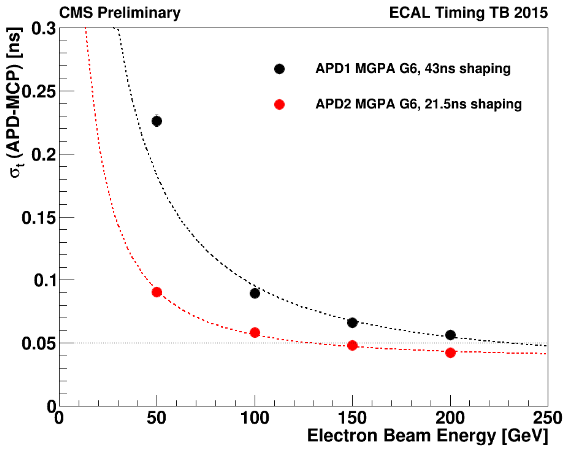
\includegraphics[width = 0.45\textwidth]{figures/upgrade/APD_t_res_vs_energy.png}
  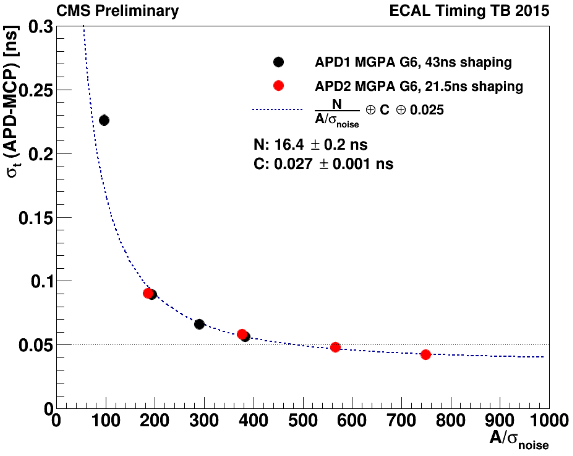
\includegraphics[width = 0.45\textwidth]{figures/upgrade/APD_t_res_vs_AoverN.png}
  \caption{Time resolution on $t_{APD}-t_{MCP}$ as a function of the beam energy (left)
    and the average signal $A/\sigma_n$ (right).
    In the left plot the lines are drawn to guide the eye while in the left plot the curve is the result of the
    fit described in the text.}
  \label{fig:results_treso}
\end{figure}

The impact of fluctuation in the light production depth on the time performance is estimated comparing the
time performance of the SiPM with that of the APDs. As illustrated in Figure~\ref{fig:light_collection_scheme}, 
the elctromagnatic shower propagates faster than the scintillation light in the crystal by a factor equal
to the \PbWO refractive index ($n=2.2$). The different propagation velocity can spoil the time resolution and the
effect is maximized when collecting the scintillation light on the front face since light produced later, deeper in
the crystal also travels a longer mimimum path to reach the photodetector on the front face than the one on the rear face.

\begin{figure}[h!]
  \centering
  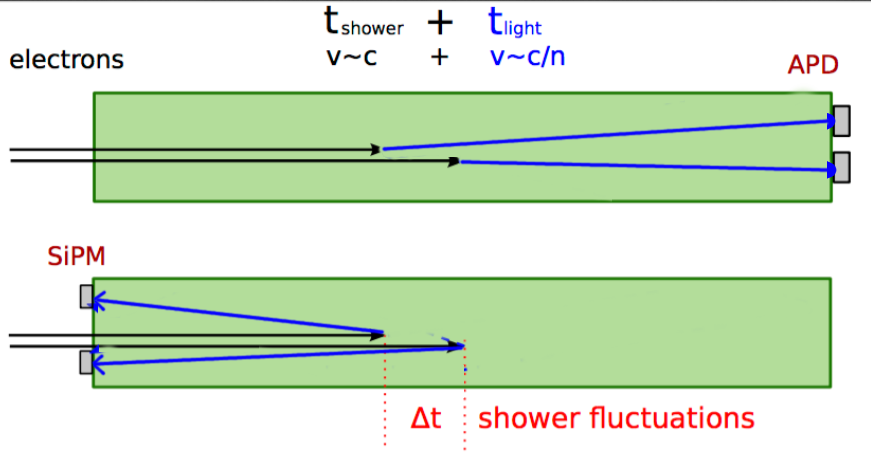
\includegraphics[width = .6\textwidth]{figures/upgrade/shower_fluct_cartoon.png}
  \caption{Illustration of light collection on the front and back face of the \PbWO crystal.}
  \label{fig:light_collection_scheme}
\end{figure}

The intrinsic time resolution of the SiPM arrays is estimeted comparing the time measured by the two different arrays using
the same procedure described for APD and MCP comparison. In this comparison shower depth fluctuations cancels since
are common to both SiPM arrays.
The result and the fit are shown in Figure~\ref{fig:sipm_tres},
the fitted time resolution constant term is 25 ps comparable to that of the APDs.
The time resolution is worse when comparing the time measured by one of the SiPM arrays to the one recorded by the MCP,
showing that fluctuation in the light emission depth impact the time resolution adding $\sim 80$ ps in quadrature regardless
of the shower energy which is clearly not affecting the APD performance.

\begin{figure}[h!]
  \centering
  \includegraphics[width = .7\textwidth]{figures/upgrade/sipm_50um_intrinsic.pdf}
  \caption{Front face light collection time performance. The times measured with the two SiPM arrays
    is compared to the MCP time (grey curves) and one to the other (red curve). SiPM time performance is comparable
    to the APDs one (red) but is affected by light emission fluctuations when comparing to an external
    reference (i.e. MCP).}
  \label{fig:sipm_tres}
\end{figure}

In 2016 a similar test was conducted with a prototype of the HL-LHC readout electronic installed in place of the
CR-RC amplification. The signal from the TIA amplifier was digitized with the same VME board used in 2015 and the
160 MHz sampling ADC is simulated at the analysis level by sampling the signal shape acquired at 5 GHz by the CAEN digitizer.
The beam test setup included also the same MCP and hodoscopes described~above. 

The event selection and time reconstruction is performed in the same way as for the 2015 beam test.
The results are reported in Figure~\ref{fig:tia_tres}: the time performance achieved by emulating the
160 MHz sampling is identical to the one obtained with 5 GHz sampling while at 80 MHz sampling the time resolution
depends on the sampling phase. ??

\begin{figure}[h!]
  \centering
  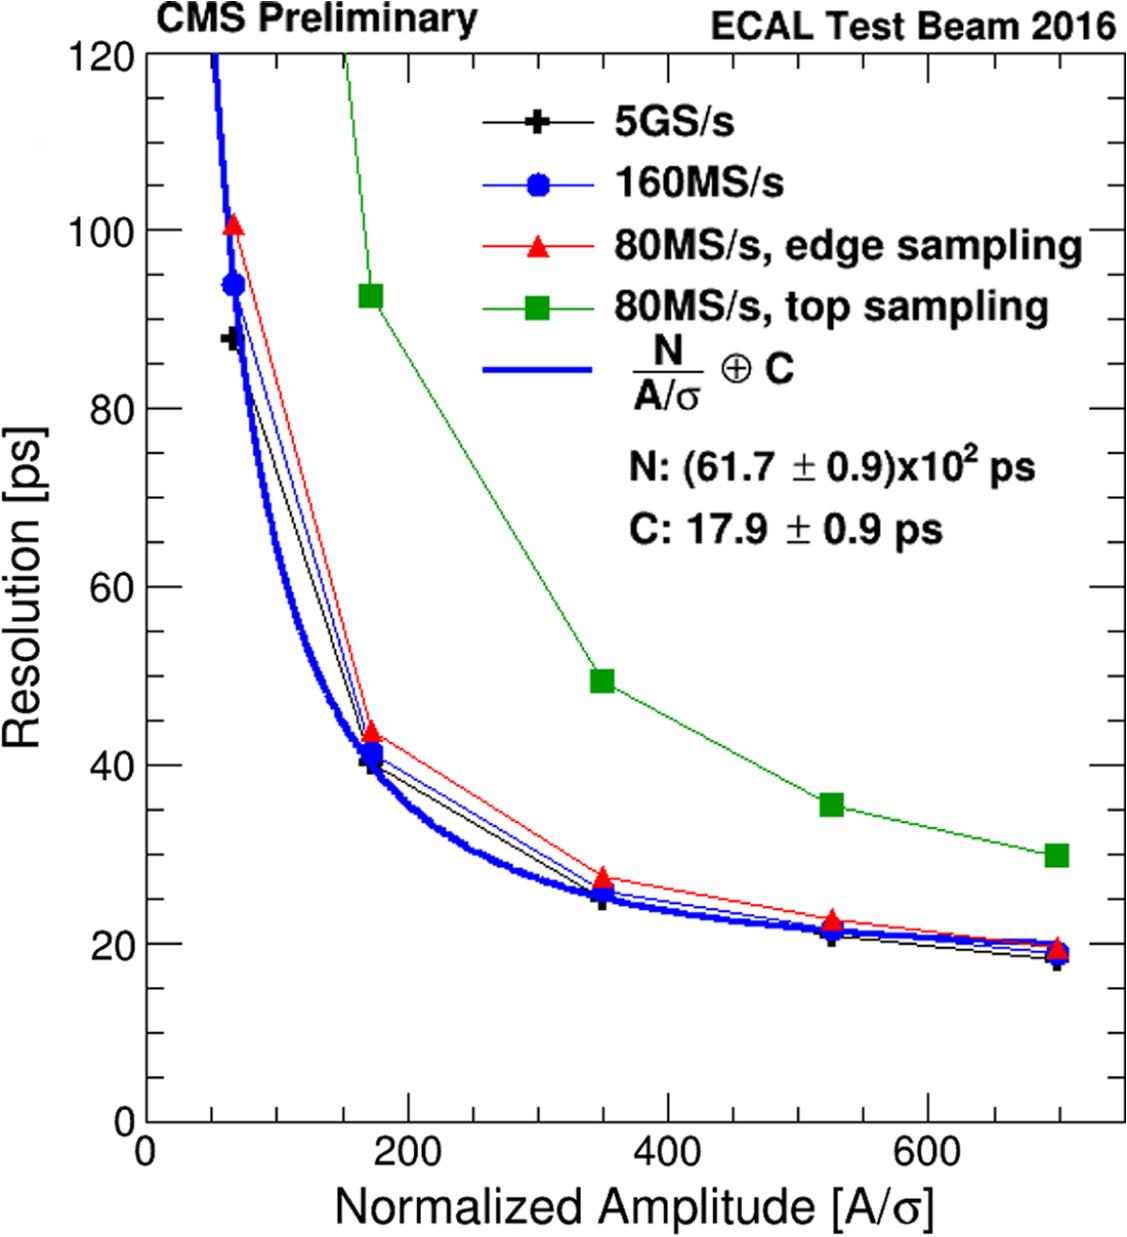
\includegraphics[width = 0.7\textwidth]{figures/upgrade/sampling_freq_res_comp.png}
  \caption{Time resolution performance of HL-LHC ECAL readout electronics for different sampling frequency.
    The baseline 160 MHz sampling frequency does not limit the time performance while the 80 MHz sampling
    performance depends on the phase between the electronics clock and the APD signal.}
  \label{fig:tia_tres}
\end{figure}
